\documentclass[letterpaper, 11pt]{article}
\usepackage[margin=1in, centering]{geometry}
\usepackage{sectsty}
\usepackage{graphicx}
\usepackage{here}
\usepackage{caption}
\usepackage{subcaption}
\usepackage{pdfpages}
\usepackage[export]{adjustbox}
\captionsetup{labelformat = empty}

% Formato: Ángel Alvarado Campos @Flutt

\begin{document}
	
	\begin{figure}[H] %Portada
		\begin{subfigure}{0.2\textwidth}
			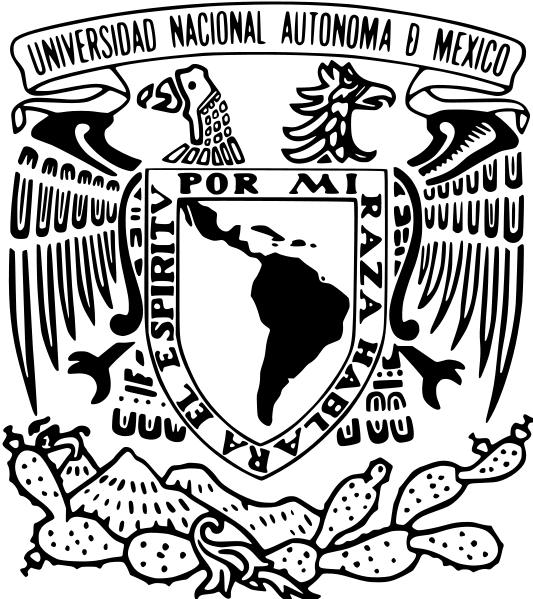
\includegraphics[scale = 0.16 ,left]{Imagenes/Portada/Escudo_UNAM.png}
		\end{subfigure}
		\hfill
		\begin{subfigure}{0.5\textwidth}
			\centering
			{\fontsize{15}{15} \selectfont Universidad Nacional Autónoma de México}
			
			\vspace{6mm}
			
			{\fontsize{15}{15} \selectfont Facultad de Ingeniería}
		\end{subfigure}
		\hfill
		\begin{subfigure}{0.2\textwidth}
			
\includegraphics[scale = 1, right]{Imagenes/Portada/Escudo_FI.jpg}
		\end{subfigure}
		
		\vspace{15mm}
		
		\centering
		{\fontsize{18}{18} \selectfont Estructuras de Datos y Algoritmos II}
		
		\vspace{25mm}
		
		{\fontsize{18}{18} \selectfont \textbf{Árboles binarios: Manual de usuario}}
		
		\vspace{20mm}
		
		{\fontsize{15}{15} \selectfont \textbf{Presenta:}}\\
		{\fontsize{15}{15} \selectfont Alvarado Campos, Ángel}\\
		
		\vspace{25mm}
		
		{\fontsize{15}{15} \selectfont \textbf{Profesor:}}\\
		{\fontsize{15}{15} \selectfont Tista García, Edgar}\\
		
		\vspace{25mm}
		
		{\fontsize{15}{15} \selectfont \textbf{Semestre:}}\\
		{\fontsize{15}{15} \selectfont 2021-1}\\
	\end{figure} %Fin Portada
	
	\newpage
	
	\section{¿Cómo iniciar?}
	
	¡Gracias por probar nuestro \textit{software}!, en esta manual le guiaremos para que le de un uso adecuado a este programa y pueda disfrutar de él.
	
	Recibirá el \textit{software} a través de una carpeta cuyo nombre es "Proyecto Adicional EDA II". Localice la carpeta y colóquela en la zona que usted guste, únicamente tenga en cuenta el directorio en que el se encontrará la carpeta.
	
	\begin{enumerate}
		\item Desde la consola de su sistema operativo, dirígase y colóquese en la carpeta "Proyecto Adicional EDA II".
		\item Dirígase a la carpeta "src".
		\item Desde "src" ejecute el comando "javac Principal/Principal.java" para \textbf{compilar}. 
		
		\begin{figure}[H]
			\centering
			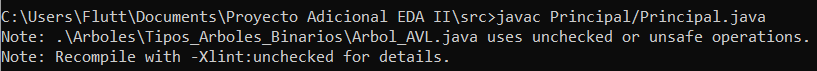
\includegraphics[scale=0.5]{Imagenes/screenshot001.png}
		\end{figure}
		
		\item[] Si se presenta un error en este proceso, ejecute "javac -Xlint Principal/Principal.java".
		
		\begin{figure}[H]
			\centering
			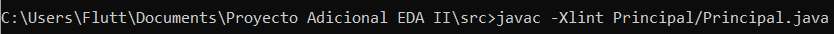
\includegraphics[scale=0.5]{Imagenes/screenshot002.png}
		\end{figure}
		
		\item Aún en "src", ejecute el comando "java Principal/Principal" para \textbf{ejecutar} el programa.
		
		\begin{figure}[H]
			\centering
			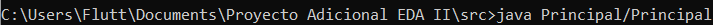
\includegraphics[scale=0.5]{Imagenes/screenshot003}
		\end{figure}
	\end{enumerate}
	
	\section{¿Cómo usar?}
	
	Al compilar el programa podrá seleccionar entre cuatro opciones: "Menu Arbol\_AVL", "Menu Heap", "Menu Arbol de expresión aritmética" y "Salir". Las tres primeras opciones le permitirán operar con estructuras de datos según lo indique el nombre. Para interactuar con el programa tendrá que introducir alguno valor entero en función de la opción que usted desee. 
	
	\begin{figure}[H]
		\centering
		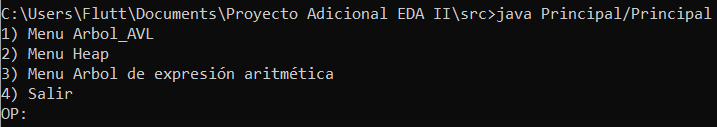
\includegraphics[scale=0.5]{Imagenes/screenshot004}
	\end{figure}
	
	Con excepción de la opción de salida, usted podrá acceder a un submenú en el que podrá operar con la estructura que desee.
	
	\newpage
	
	\section*{Menú Arbol\_AVL}
	
	Si selecciona la opción 1 desde el menú principal podrá ingresar al menú para operar con un árbol autobalanceado y se mostrarán 6 opciones:
	
	\begin{figure}[H]
		\centering
		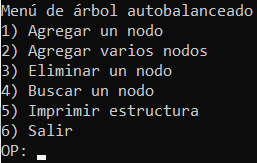
\includegraphics[scale=0.5]{Imagenes/screenshot005}
	\end{figure}
	
	\begin{enumerate}
		\item Agregar un nodo: Añadir un nodo de manera individual al 
		árbol. Se le solicitará ingresar el valor entero que desea añadir.
		
		\begin{figure}[H]
			\centering
			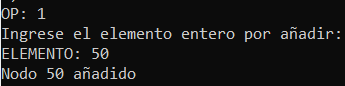
\includegraphics[scale=0.5]{Imagenes/screenshot006}
		\end{figure}
		
		
		\item Agregar varios nodos: Añadir varios nodos en una misma instrucción. Todos los valores tendrán que enlistarse separados por espacios en blanco. Si se tiene algún nodo repetido, éste no se añadirá, pero si los demás.
		
		\begin{figure}[H]
			\centering
			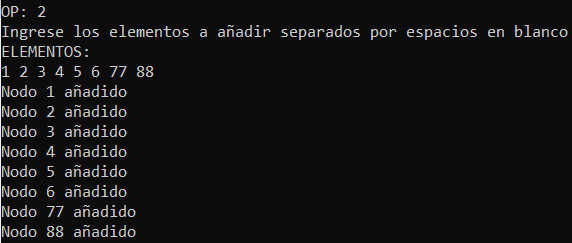
\includegraphics[scale=0.5]{Imagenes/screenshot007}
		\end{figure}
		
		\item Eliminar un nodo: Eliminar un nodo del árbol siempre y cuando exista. Se le solicitará ingresar el valor entero del nodo que desea eliminar.
		
		\begin{figure}[H]
			\centering
			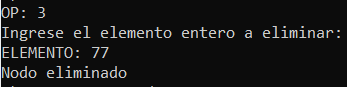
\includegraphics[scale=0.5]{Imagenes/screenshot008}
		\end{figure}
		
		\item Buscar un nodo: Realizar la búsqueda de un nodo en el árbol. 
		
		\begin{figure}[H]
			\centering
			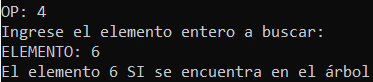
\includegraphics[scale=0.5]{Imagenes/screenshot009}
		\end{figure}
		
		\item Imprimir estructura: Imprimir a cada uno de los nodos involucrados en el árbol junto con sus hijos. La clave "I" indica el hijo izquierdo, mientras que "D" lo que hace con el derecho.
		
		\begin{figure}[H]
			\centering
			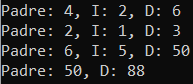
\includegraphics[scale=0.5]{Imagenes/screenshot010}
		\end{figure}
	\end{enumerate}

	\newpage
	
	\section*{Menú Heap}
	
	Si selecciona la opción 2 desde el menú principal podrá ingresar al menú para operar con una estructura \textit{heap} y se mostrarán 5 opciones:
	
	\begin{figure}[H]
		\centering
		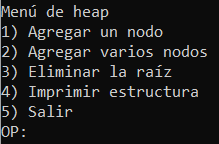
\includegraphics[scale=0.5]{Imagenes/screenshot011}
	\end{figure}

	\begin{enumerate}
		\item Agregar un nodo: Añadir un nodo de manera individual al 
		árbol. Se le solicitará ingresar el valor entero que desea añadir.
		
		\begin{figure}[H]
			\centering
			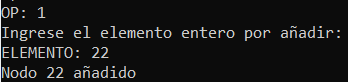
\includegraphics[scale=0.5]{Imagenes/screenshot012}
		\end{figure}
		
		\item Agregar varios nodos: Añadir varios nodos en una misma instrucción. Todos los valores tendrán que enlistarse separados por espacios en blanco. Si se tiene algún nodo repetido, éste no se añadirá, pero si los demás.
		
		\begin{figure}[H]
			\centering
			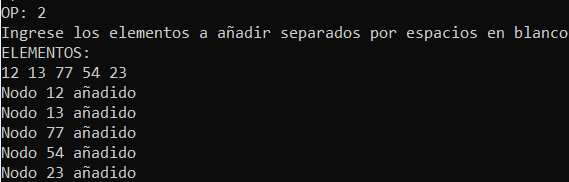
\includegraphics[scale=0.5]{Imagenes/screenshot013}
		\end{figure}
	
		\item Eliminar la raíz: Eliminar al nodo raíz actual del árbol. No se le solicitará ingresar algún elemento, el programa sabe qué hacer. 
		
		\begin{figure}[H]
			\centering
			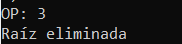
\includegraphics[scale=0.5]{Imagenes/screenshot014}
		\end{figure}
		
		\item Imprimir estructura: Imprimir a cada uno de los nodos involucrados en el árbol junto con sus hijos. La clave "I" indica el hijo izquierdo, mientras que "D" lo que hace con el derecho.
		
		\begin{figure}[H]
			\centering
			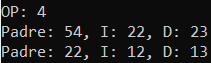
\includegraphics[scale=0.5]{Imagenes/screenshot015}
		\end{figure}
		
	\end{enumerate}
	
	\newpage
	
	\section*{Menu Arbol de expresión aritmética}
	
	Si selecciona la opción 3 desde el menú principal podrá ingresar al menú para operar con un árbol de expresión aritmética a partir de una expresión que usted ingrese:
	
	\begin{figure}[H]
		\centering
		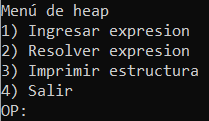
\includegraphics[scale=0.5]{Imagenes/screenshot016}
	\end{figure}
	
	\begin{enumerate}
		\item Ingresar expresión: Podrá ingresar una operación aritmética que cumpla siempre con las siguientes propiedades: 
		\begin{enumerate}
			\item Operar únicamente con número enteros unitarios. Es decir, enteros en el rango de $[0,9]$
			\item Todas las operaciones deben ser totalmente binarias, es decir, si los operandos no son elementos simples, estos tendrán que encontrarse encerrados en paréntesis. Por ejemplo: "((5+2)*(3-1))" o "((3-2)*((2*1)-(4/2)))".
			\item Toda la expresión debe estar encerrada en un paréntesis global para ser leída. Esto se observa en los dos ejemplos anteriores.
			
			\item[\textbf{*}] \textbf{IMPORTANTE}: Si no se cumple con las propiedades anteriores, el programa presentará un error y no ejecutará la expresión.
		\end{enumerate}
		
		\begin{figure}[H]
			\centering
			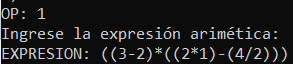
\includegraphics[scale=0.5]{Imagenes/screenshot017}
		\end{figure}
		
		\item Resolver expresión: Si la expresión fue ingresada correctamente, podrá ver el resultado con esta opción.
		
		\begin{figure}[H]
			\centering
			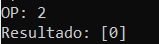
\includegraphics[scale=0.5]{Imagenes/screenshot018}
		\end{figure}
		
		\item Imprimir estructura: Imprimir a cada uno de los nodos involucrados en el árbol junto con sus hijos. La clave "I" indica el hijo izquierdo, mientras que "D" lo que hace con el derecho.
		
		\begin{figure}[H]
			\centering
			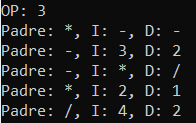
\includegraphics[scale=0.5]{Imagenes/screenshot019}
		\end{figure}
		
	\end{enumerate}
	
	\newpage
	
	\section*{Notas generales}
	
	\begin{enumerate}
		\item Si se encuentra en cualquier submenú y selecciona la opción que corresponde a salir, el árbol construido en la ejecución se eliminirá.
		\item Se recomienda que ingrese únicamente las opciones que se le muestran en el menú. Todo esta controlado ante cualquier imprevisto del usuario, pero se le recomienda qu no lo haga.
		\item El instructivo se llevó a cabo considerando un equipo con sistema operativo Windows 10.
	\end{enumerate}
	
\end{document}}